\section{Introduction}
\label{sec:introduction}

The Border Gateway Protocol (BGP)~\cite{rfc4271} is the routing foundation of the global Internet, enabling independently operated autonomous systems (ASes) to exchange reachability information for IP prefixes. Yet BGP has no route origin authentication and cannot verify whether an AS is authorized to originate a prefix~\cite{rfc4272,kent2000sbgp}. This gap leaves interdomain routing vulnerable to accidental misoriginations and malicious prefix hijacks that can divert, intercept, or disrupt traffic~\cite{ballani2007hijacking,butler2010bgp}.

To address this gap in origin authorization, the IETF specified the Resource Public Key Infrastructure (RPKI) architecture~\cite{rfc6480} and standardized a profile for Route Origin Authorizations (ROAs)~\cite{rfc9582}. Prefix holders publish ROAs to identify the ASes authorized to originate their prefixes. Routers then use the published ROAs to determine whether the origin of a BGP route is authorized, a process known as Route Origin Validation (ROV)~\cite{rfc6811,rfc8481}. For a route covered by at least one ROA, ROV checks whether a covering ROA authorizes its origin AS and permits its prefix length. If none does, ROV classifies the route as \invalid{}. Depending on local routing policy, an \invalid{} route may be rejected or assigned a lower preference.

An \invalid{} result indicates a conflict with the published ROAs, but not by itself malicious intent~\cite{chung2019,xu2019falsealarm,schulmann2025learning}. A 17-month study classified at least 91\% of daily \invalid{} routes as harmless, and its routing table analysis suggests that rejecting all such routes can eliminate alternative paths and, in some cases, render prefixes unreachable~\cite{righttheship2025}. Transit and IP leasing workflows recur as sources of persistent ROA mismatches, where announcements can precede ROA updates during manual coordination~\cite{demystifying2026}. Intended routing changes can therefore precede a matching ROA: limited visibility of a downstream origin choice creates this gap, and manual reporting extends it. During the gap, ROV labels the intended route \invalid{}, and a policy that filters it can impair reachability.

We focus on a setting in which policy must be installed before the holder knows which origin AS will originate a particular proper subprefix~\cite{demystifying2026,leasing2026}. Figure~\ref{fig:motivation} contrasts the two options available to the holder. Issuing the aggregate ROA, as in Case~1, keeps the aggregate \valid{} but makes a later proper subprefix with a different origin \invalid{}, because no ROA matches that subprefix. Withholding the ROA, as in Case~2, leaves both the aggregate and the subprefix \notfound{}. Conventional ROV therefore cannot keep the aggregate authorized and admit the later route.

\begin{figure}[tb]\centering
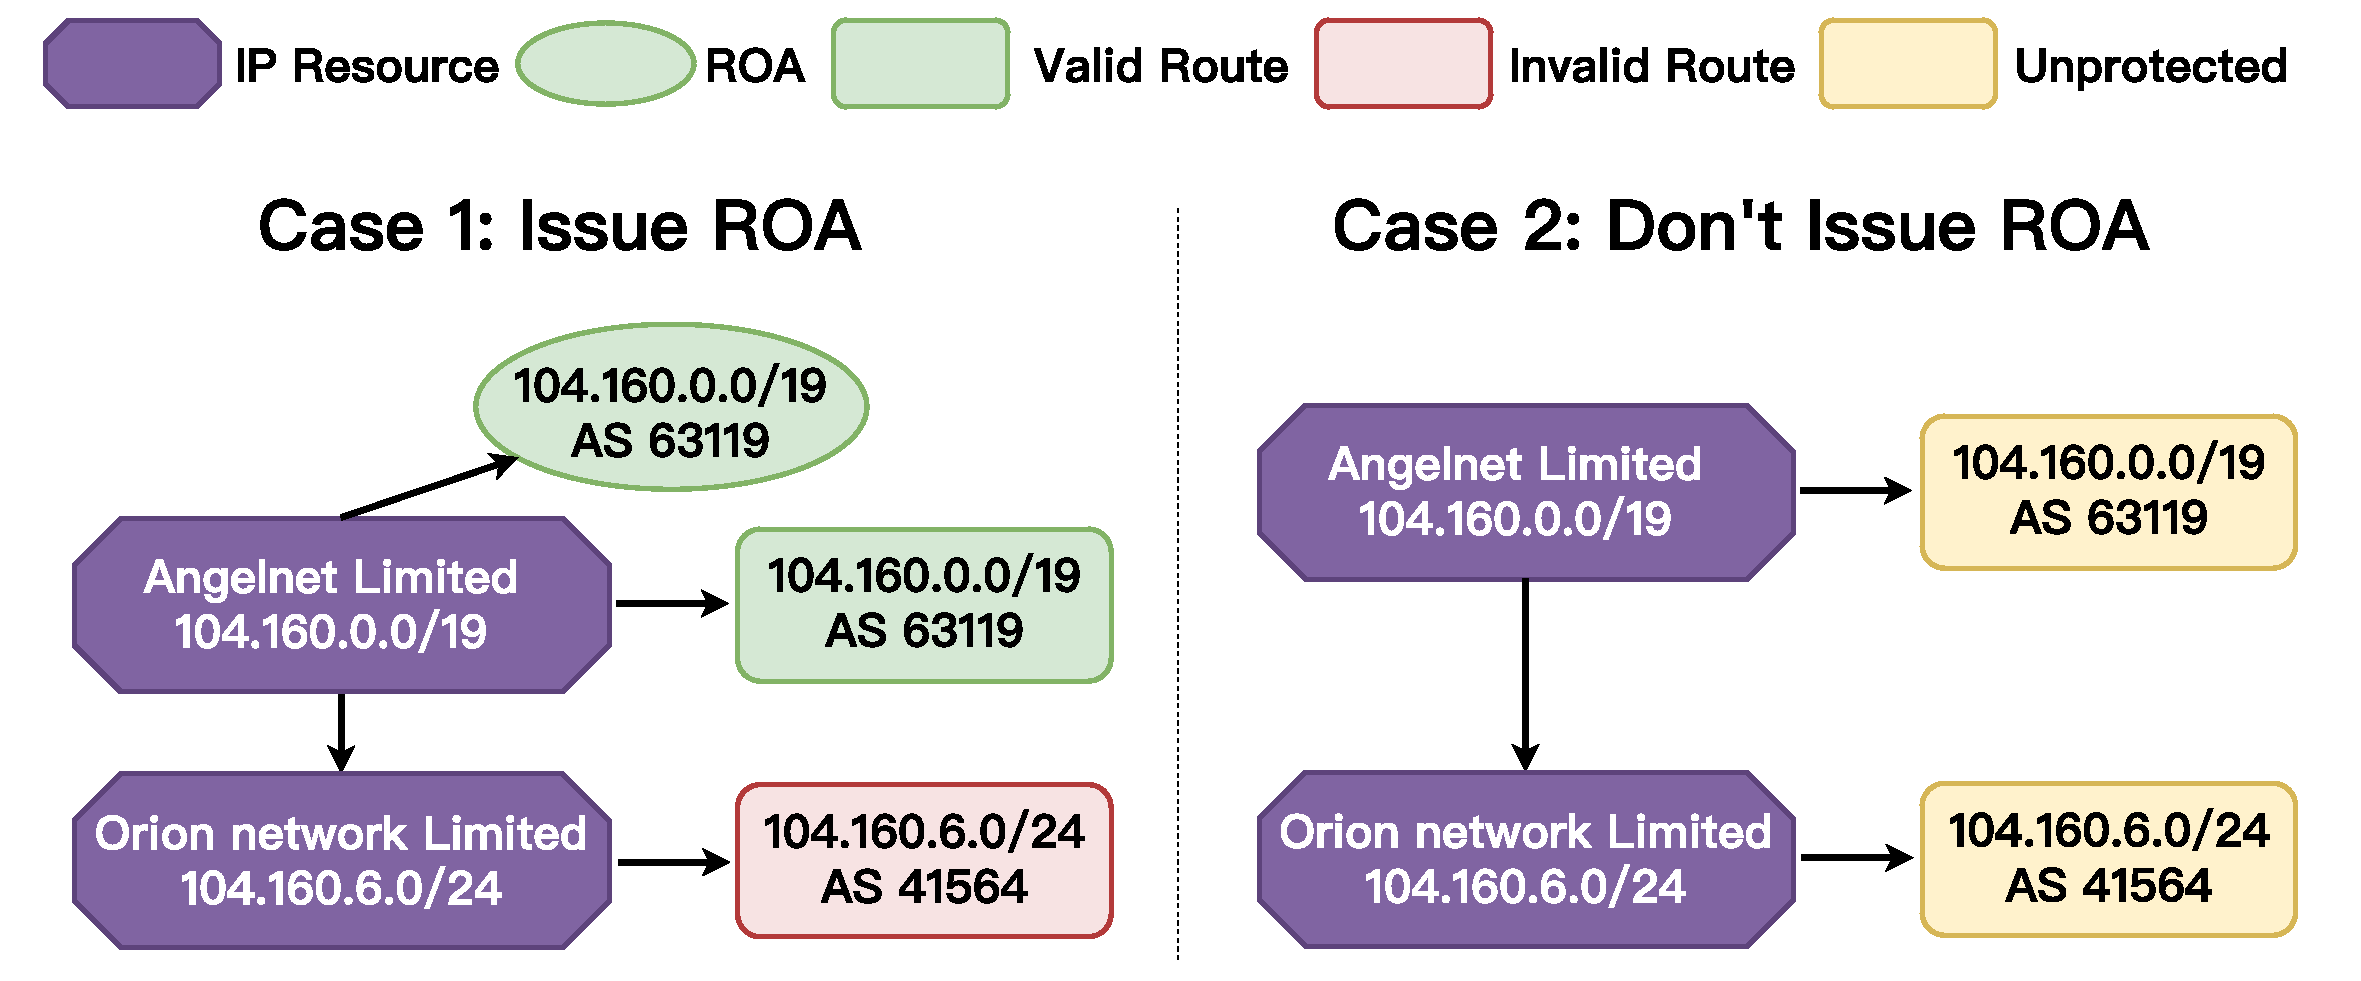
\includegraphics[width=\columnwidth]{figures/fig_motivation}
\caption{Aggregate--subprefix authorization dilemma.}
\label{fig:motivation}\end{figure}

Broadening \emph{maxLength} does not resolve the dilemma because it extends the allowed prefix lengths only for the origin already listed in the ROA~\cite{rfc9319,rfc9582}. An operator can configure local routing policy not to filter the route or use SLURM to override its local RPKI view, but neither approach provides portable policy signed by the holder~\cite{rfc7115,rfc8416}. The wildcard ROA proposal authorizes any AS at its target prefix. Until a regular ROA is issued, a hijacker can therefore announce that prefix and still pass origin validation~\cite{gilad2017rpki}.

In this paper, we introduce Subprefix-Scope ROV (\ssrov{}) to retain explicit origin authorization for an aggregate route with a known origin. It does so without listing every future proper subprefix origin in advance. The holder instead publishes a signed policy that identifies proper-subprefix regions and sets a maximum route-prefix length. If a later route is covered only by this policy, \ssrov{} labels it \openscope{} instead of \invalid{}. Operators can then apply a separate local routing policy to \openscope{} routes, without waiting for reactive publication of an exact ROA.

{\revstart Admitting an intended route in this way also admits an eligible origin that the holder did not select. \ssrov{} records that a route lies below a holder-signed marker and within the policy's length bound; it does not record that the origin is authorized. We therefore present \ssrov{} as a bounded security--availability trade-off rather than as a hijack defense: during the gap, an adversary announcing from an eligible AS inside a marked region receives the same state as the intended origin, and only the local action separates them. Section~\ref{sec:security-scope} states the adversary model, and Section~\ref{sec:eval-security} measures the exposure it creates.}

This paper makes three contributions.
\begin{itemize}
\item We formalize why conventional ROV cannot simultaneously protect an aggregate with a known origin and avoid classifying an unmatched proper subprefix with a different origin as \invalid{} when the downstream origin choice is not yet visible to the issuer.
\item We design \ssrov{}, in which the holder signs prefix markers and a maximum route-prefix length, but no downstream origin list. It preserves conventional ROV semantics and separates the aggregate's \explicit{} state from an eligible descendant's \openscope{} state, making it strictly more expressive for this dilemma.
\item \rev{We ground the problem in observed allocation paths and evaluate an IPv4 and IPv6 prototype across conflicts during partial ROA issuance, system cost, intended-route delivery, unlisted-origin exposure, and the reachability an adversary gains inside a marked region.}
\end{itemize}

To support reproducibility, the implementation, experiment and analysis scripts, configurations, result tables, and figure source data are available at \url{https://github.com/chenyxuan/s2rov-artifact}.

The remainder of the paper is organized as follows. Section~II formalizes the aggregate--subprefix gap and examines downstream-origin visibility and observed allocation paths. \rev{Section~III presents the \ssrov{} design and its security scope, and Section~IV describes the prototype. Section~V reports the evaluation, including the exposure a marked region creates. Sections~VI and~VII discuss related work and the scope of the evidence, respectively, and Section~VIII concludes the paper.}
